\section{\LaTeX}

%-----------------------    ---------------------------------

\begin{frame}
\frametitle{¿Qué es \LaTeX ?}

\begin{itemize}
   \item Sistema de composición de textos
   \item \LaTeX\ en realidad es un conjunto de scripts para facilitar el uso del lenguaje de composición tipográfica \TeX\ creado por Donald Knuth
   \item No es WYSIWYG, sino que se basa en instrucciones
   \item Se compila, para obtener el resultado final (generalmente, un PDF)
   \item (aunque hay editores \LaTeX\ WYSIWG, como LyX)
   \item Ventajas:
   \begin{itemize}
     \item Separa visualización de contenido
     \item Gestión de referencias (a figuras, tablas, capítulos...)
     \item Tablas de contenidos, figuras y tablas generada automáticamente
     \item Gestión bibliográfica
     \item Fórmulas matemáticas, caracteres especiales...
     \item Es texto plano... ideal para \texttt{grep} y \texttt{GitHub}
   \end{itemize}
\end{itemize}

\end{frame}

%-----------------------    ---------------------------------

\begin{frame}
\frametitle{¿Para qué se utiliza \LaTeX ?}

\begin{itemize}
   \item Se utiliza mucho en textos científico técnicos
   \item Por ejemplo, puedes utilizarlo para escribir la memoria de tu Trabajo Fin de Grado. Tienes una plantilla disponible en \url{https://github.com/gregoriorobles/plantilla-memoria}
   \item En GSyC las utilizamos para nuestras transparencias (¡Estas transparencias están hechas en \LaTeX\ (con Beamer)!)
\end{itemize}

\end{frame}


%-----------------------    ---------------------------------

\begin{frame}
\frametitle{Flujo de trabajo en \LaTeX}

\begin{center}
  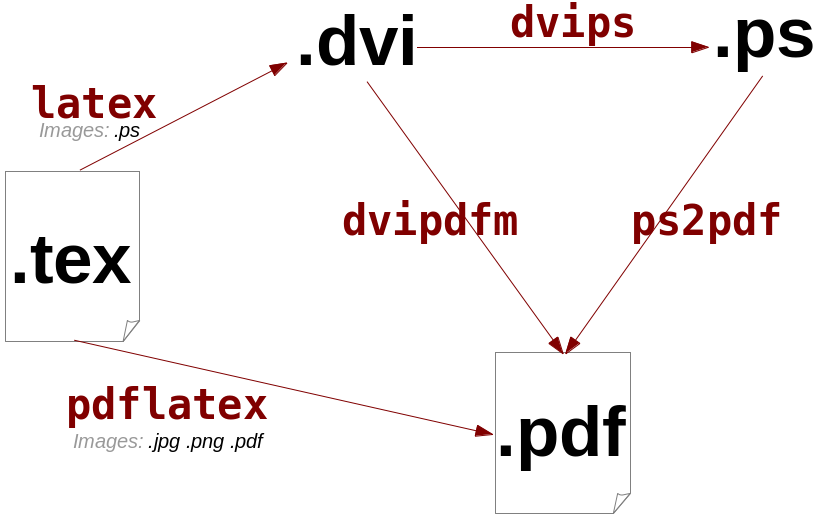
\includegraphics[width=8cm]{figs/latex.png}
\end{center}


\begin{flushright}
{\tiny
Fuente: Wikipedia (Creative Commons Attribution-ShareAlike)
}
\end{flushright}

\end{frame}


